\documentclass[a4paper]{usiinfbachelorproject}

\captionsetup{labelfont={bf}}
%%%%%%%%%%%%%%%%%%%%%%%%%%%% PACKAGES %%%%%%%%%%%%%%%%%%%%%%%%%%%%%
\usepackage{float}
\usepackage{amsmath}


\usepackage[utf8]{inputenc}



%%% Main Body %%%

\author{Robert Jans}

\title{\textbf{Implementing GPS Spoofing Detection in a Software Receiver}}
%\subtitle{Subtitle}
\versiondate{\today}

\begin{committee}
%With more than 1 advisor an error is raised...: only 1 advisor is allowed!
\advisor[Universit\`a della Svizzera Italiana, Switzerland]{Prof.}{Miroslaw}{Malek}
%You can comment out  these lines if you don't have any assistant
\coadvisor[Universit\`a della Svizzera Italiana, Switzerland]{Dr.}{Alberto}{Ferrante}

\end{committee}

\abstract { \emph{Global Navigation Satellite System} (GNSS) receivers are nowadays used in many applications, ranging from
personal navigation devices to spacecraft navigation. Therefore, reliable GNSS positioning is fundamental and
failure to provide accurate positioning could cause catastrophic effects
threatening vital infrastructures and even causing loss of human lives.
There may be different reasons for unreliable GNSS signals, among which
malicious attacks. A preliminary study was performed at USI on
detection of spoofing attacks to \emph{Global positioning system} (GPS) signals based on machine learning
methods. These methods can detect spoofing attacks, and even classify
them in three categories, with very high accuracy. The goal of this project is to implement
one of these detection methods and integrate it into an existing open source 
\emph{Software Defined Receiver}(SDR), namely \href{https://gnss-sdr.org/}{GNSS-SDR}.
\\ \\
\textbf{Keywords}: GNSS; GPS; Spoofing Detection

}
\begin{document}
\maketitle
\tableofcontents\newpage
%\listoffigures\newpage

\section{\textbf{Introduction}}

GNSS systems are able to determine a receiver's position by comparing time signals emitted by satellites. Basically
from the time differences the distance of a satellite can be calculated, then the position is computed using triangulation of the distances to several satellites. A detailed description of the inner workings of GNSS systems goes beyond the scope of this project, but useful information can be found e.g. on 
\href{https://en.wikipedia.org/wiki/Satellite\_navigation}{Wikipedia}.

In real-world application there are two fundamentally distinct kinds of GNSS receivers: hardware receivers and software defined receivers. Both give as output an estimate of the receiver's position in terms of longitude, latitude and height
(in some cases also velocity and acceleration are determined), in addition to some metadata including timestamps; the difference lies in the implementation: in the former kind the algorithms needed for extrapolating the positioning data
from the raw signals are built into the hardware of an embedded device, while in the latter kind the raw signals are given as input to a software program which performs the post-processing.

This project focuses on a software defined receiver for the main reason that it is easily modifiable, so the
spoofing detection feature can be implemented by writing software to be integrated into the existing program.
The choice of using GNSS-SDR is based on the the fact that it is open-source and widely used for research purposes. 

The final result is a modified version of GNSS-SDR which adds a warning message to its output in case a spoofing attack is detected.


\section{\textbf{Background}}

The project builds upon research conducted at the \emph{Advanced Learning and Research Institute} (ALaRI), Faculty of Informatics, Università della Svizzera italiana (USI).
The main reference and staring point of my work is the report 
"GAD: Machine Learning GNSS Attack Detection" proposed in 2017 by Dr. Alberto Ferrante.

The GAD report describes several methods for spoofing detection based on classifiers which take as input features 
some properties of the raw signals as well as some of the processed data.

Due to the limitations in development time, this project considers only one
of them: The J48 decision tree which gave best results on general attack detection.
 Future work may include the integration of other classifiers in order to distinguish the different attack types.

\textbf{J48} is a general purpose decision tree algorithm implemented in Java and included in the \href{https://www.cs.waikato.ac.nz/ml/weka/index.html}{WEKA}
project. J48 is an implementation of the C4.5 algorithm developed in 1993 by Ross Quinlan \cite{QUINLAN}, 
who published a book about it in 1993 . A review of the book consisting in a description of the algorithm was written by Steven L. salzberg \cite{SALZBERG}.

Much of my implementation is inspired by a comparative study published
by H. M. E. Hssina, which describes in detail the algorithm and compares it with its predecessor ID3 \cite{HSSINA}.




	\subsection{\textbf{High-level structure of GNSS-SDR}}
	
GNSS-SDR is a software written in C++ which is able to process several channels of GNSS data in parallel. It
has a modular structure which makes it highly configurable (e.g. for using different signal sources). At a high level
the program can be described as a sequence of processing blocks implementing a data flow architecture. \\

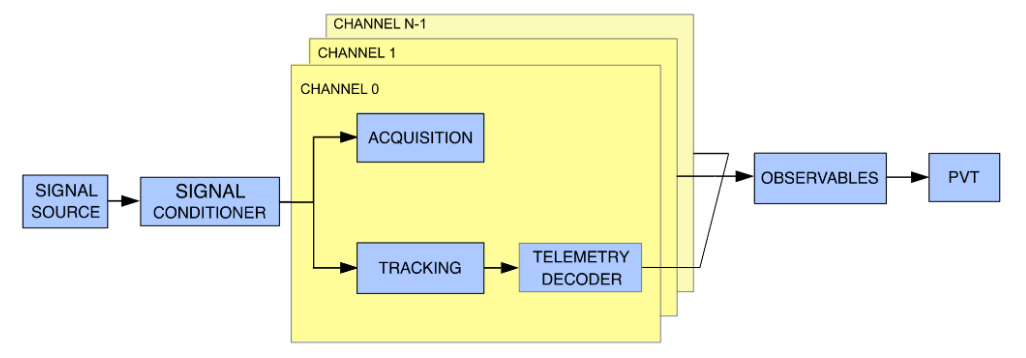
\includegraphics[width=.8\linewidth]{figures/gnss_structure} \\

For each block there are several implementations; which implementation to use at which processing stage can
be defined in a configuration file. For instance as signal source implementations there are available modules
designed for specific hardware front-ends as well as file signal sources (For this project
only file signal sources are used, but as a further work it could be considered to test the system with real time signals and spoofing devices).

	\subsection{\textbf{Retrieving the features for the classifier}}
	
In GNSS-SDR after the acquisition stage, per-channel information is stored and updated in an object of a class called
Gnss\_Synchro and propagated through the blocks up to the PVT, where the output is generated. The original version
of Gnss\_Synchro already contains some features needed, or information based on which the features can be computed.
An important exception is the amplitude of the raw signal, which is available at the acquisition stage but not
stored in the Gnss\_Synchro. the strategy to deal with this issue is to add a field to the mentioned class
in order to store and propagate the missing information. 

With this setting all features needed for the classifier can be retrieved from the Gnss\_Synchro objects at the PVT stage. More on this will follow in the section dedicated to the implementation.


	\subsection{\textbf{The C4.5 decision tree algorithm}}
	
	\subsubsection{\textbf{About decision trees}}
	
Decision trees are popular tools in machine learning and data mining, mainly due to their
simplicity and efficiency: though being structurally simple and not not
excessively expensive in terms of computational time, they often return good results
on data based classification problems.
The basic concept is to start with a root node containing the entire training
set and splitting it on some criteria. the process then is carried out recursively
on the child nodes until some base case is reached; at this point a lea node representing
a decision is created.

The C4.5 algorithm uses the information theoretical concept of entropy as splitting criterion: the set is split based on the feature that provides the greatest amount of information about the set with respect to the classification.
	
	\subsubsection{\textbf{Concepts from information theory}}
	
C4.5 uses the concepts of \emph{Entropy} and \emph{Gain},
which are defined as follows:

\begin{description}

	\item[Entropy]
	given a probability distribution $P$ and a sample $S$ of size $n$
	$$H(P) = - \sum_{i=1}^n p_i \cdot \log_2 (p_i)$$
	
	\item[Gain]
	With $D$ being the the set to split and $D_1$, $D_2$ the candidate subsets,
	the gain is the difference in of the entropy of $D$ and the weighted
	sum of the entropies of $D_1$ and $D_2$:
	$$G(D, D_1, D_2) = H(D) - H(D_1)\cdot \frac{|D_1|}{|D|} - H(D_2) \cdot \frac{|D_2|}{|D|}$$
	
\end{description}

In the C4.5 the gains must be calculated for splits on all possible
attribute-value pairs, the pair which leads to the highest gain is
selected as decision condition for the given node.

	\subsubsection{\textbf{Steps of the algorithm}}
	
\begin{description}

	\item[base case 1]
	all elements of the set belong to the same class: create
	a leaf with the given class as decision result.
	
	\item[base case 2]
	the gain is zero or below a defined threshold:
	transform the parent node into a leaf, with the majority class as 
	decision value.
	
	\item[base case 3 (optional)]
	the tree has reached a defined maximum depth: create a leaf node with the majority class as 
	decision value.
	
	\item[base case 4 (optional)]
	the set is smaller than a defined minimum size: create a leaf node as above.

	\item[recursive case]
iterate over all attributes, for each attribute iterate over the values. for
each attribute-value pair compute the gain and choose the best one.
Apply the procedure to the two subsets obtained by splitting on the selected attribute-value pair.

Every time an attributeis selected remove it from the attributes on which to test in the child nodes.

\end{description}

	\subsection{\textbf{The TEXBAT data set}}
	
the \emph{Texas Spoofing Test Battery} TEXBAT is a set of recorded spoofed and non spoofed GNSS traces which is freely
available at \href{http://radionavlab.ae.utexas.edu/datastore/texbat/}{http://radionavlab.ae.utexas.edu/datastore/texbat/}.
The data used for training, valdating and testing of this project's implementations is taken from parts of TEXBAT.

Researchers at the ALaRI institute have prepared csv files containing records from TEXBAT labeled as "spoofed" or
"clean", which is the basis for the supervised learning procedure.






\section{\textbf{Approach}}

	\subsection{\textbf{General outline}}

The main part of my work is extracting the required features from GNSS-SDR, building a special purpose C++ version of the algorithm, adapted to the specific features used in the ALaRI research, and integrate it into GNSS-SDR.

In order to train the classifier, ALaRI provided a labeled data-set based on \emph{TEXBAT} for supervised learning. In order to achieve 
a light-weight implementation capable of running on embedded devices with limited resources, the idea is to build the
decision tree offline and encode it in a file, from which a minimal tree (containing only the decision attribute and threshold value for each node) can be loaded to run in real-time.
		
	\subsection{\textbf{Feature retrieval}}
	
For using a classifier, at some point in the data flow of GNSS-SDR all the required features need to be assembled
and made available to the classifier. In the case treated by this project (corresponding to the tests made at ALaRI
using J48 with16 features), the following features are needed:

\begin{itemize}

\item
minimum Doppler

\item
average Doppler

\item
standard deviation of Doppler

\item
minimum number of valid satellites

\item
average number of valid satellites

\item
standard deviation of the number of valid satellites

\item
maximum number of satellites changed

\item
standard deviation of the number of satellites changed

\item
minimum signal to noise ratio

\item
maximum signal to noise ratio

\item
average signal to noise ratio

\item
standard deviation of signal to noise ratio

\item
minimum pseudorange

\item
average pseudorange

\item
standard deviation of pseudorange

\item
maximum carrier phase

\end{itemize}

At the PVT processing stage some of these features are available in the incoming Gnss\_Synchro objects,
others are available in the PVT output, yet others can be computed either by combining available values or keeping track of values over time (for minima, maxima, averages and standard deviations). Details are described in the implementation section.
		
		
	\subsection{\textbf{Building the C4.5 decision tree}}
	
A separate program takes as input the csv containing the labeled data and outputs a file containing an encoded form of the decision tree. The program must be able to run independently from GNSS-SDR since the processing time can be large given
large input files.

	\subsection{\textbf{Create and integrate the classifier}}
	
A program representing the decision tree must be built given a file with the encoded tree. This program must use the features extracted at run-time and provide a classification decision. It needs to interact directly with GNSS-SDR in order
to include warnings in the outputs of the PVT.
	
	\subsection{\textbf{Validation and testing}}
	
in order to tune the hyper-parameters of the tree-generating program, experiments need to be done on a validation set.
Performance assessments are to be done on a separate testing data set. Luckily the available data-set is large enough
to allow splitting it into disjoint subsets, leaving the training set large enough.
		
		
\section{\textbf{Implementation}}

\subsection{Making the features available at the PVT level of GNSS-SDR.}

\subsubsection{Propagating the raw signal amplitude information from acquisition to PVT}

Though in the end the amplitude of the raw signal is not among the features used by the classifier 
built in this project, it might be useful in further works when implementing other classifiers.

TODO: describe mods on Gnss\_Synchro.

\subsection{Tree construction}

\subsubsection{Differences with respect to the original C4.5 algorithm}

\subsection{Classifier construction}

\subsubsection{Training and testing on the provided csv files}

\subsection{Integration into GSS-SDR}

\subsubsection{Testing on TEXBAT data}

Running the system on a set of spoofed signals(\texttt{ds7.bin}) classified as expected all traces
as spoofed. Unexpected was in stead the behavior on a clean data set (\texttt{cleanStatic.bin}):
all records were wrongly classified as spoofed. There clearly is a mismatch between the provided csv data 
and the data extracted by the \texttt{FeatureSet} class I wrote. One possibility is that there is a bug in the extraction
procedure, an other one is that the provide csv data were somehow pre-processed.

A reasonable strategy to investigate this situation is to write an extension to the feature extractor which
produces csv files containing the data extracted, training classifier on these files and check whether the results are better.







\section{\textbf{Evaluation}}
	\subsection{\textbf{Results}}
	The experimental result goes here ... \footnote{https://www.usi.ch}. \\
	
 
TO BE DONE




		
\newpage
\section{\textbf{Future work}}

\section{\textbf{Summary}}
Future works goes here.






\newpage
	
%%%%% BIBLIOGRAPHY %%%%%
\bibliographystyle{abbrv}
\bibliography{references}


\end{document}
